\documentclass[tikz,border=2pt]{standalone}
\usepackage{amsmath,amssymb}
\usepackage{tikz}

\begin{document}
% Three inventory settings of the course: constant demand (EOQ sawtooth, order a fixed
% quantity when stock hits zero), known varying demand per period (dynamic lot sizing) and
% random single-period demand (newsvendor: one stock quantity chosen before demand is seen).
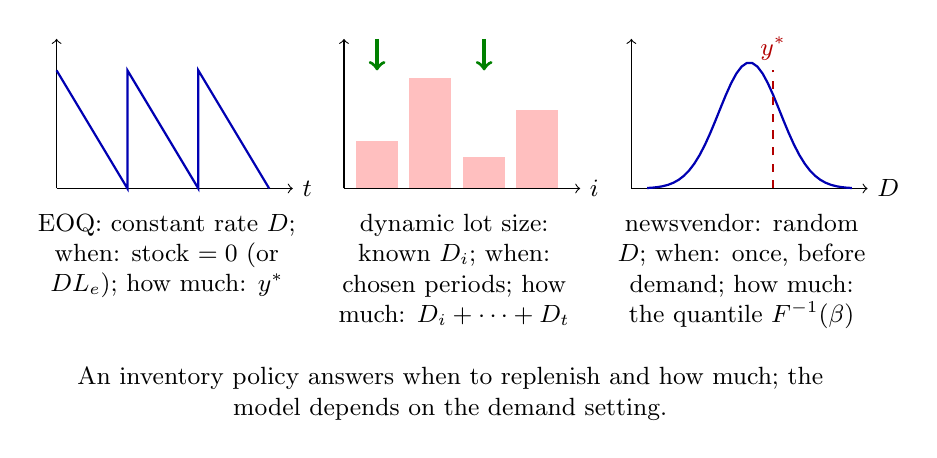
\begin{tikzpicture}[every node/.style={font=\small}]
	\begin{scope}
		\draw[->] (0,0) -- (3.0,0) node[right] {$t$};
		\draw[->] (0,0) -- (0,1.9);
		\draw[blue!70!black, thick] (0,1.5) -- (0.9,0) -- (0.9,1.5) -- (1.8,0) -- (1.8,1.5) -- (2.7,0);
		\node[anchor=north, align=flush center, text width=3.3cm] at (1.4,-0.2) {EOQ: constant rate $D$; when: stock $=0$ (or $DL_e$); how much: $y^*$};
	\end{scope}
	\begin{scope}[xshift=3.65cm]
		\draw[->] (0,0) -- (3.0,0) node[right] {$i$};
		\draw[->] (0,0) -- (0,1.9);
		\foreach \i/\d in {0/0.6, 1/1.4, 2/0.4, 3/1.0} {\fill[red!25] ({0.15+0.68*\i},0) rectangle ({0.68+0.68*\i},\d);}
		\draw[green!50!black, very thick, ->] (0.42,1.9) -- (0.42,1.5); \draw[green!50!black, very thick, ->] (1.78,1.9) -- (1.78,1.5);
		\node[anchor=north, align=flush center, text width=3.3cm] at (1.4,-0.2) {dynamic lot size: known $D_i$; when: chosen periods; how much: $D_i+\dots+D_t$};
	\end{scope}
	\begin{scope}[xshift=7.3cm]
		\draw[->] (0,0) -- (3.0,0) node[right] {$D$};
		\draw[->] (0,0) -- (0,1.9);
		\draw[blue!70!black, thick, domain=0.2:2.8, samples=40] plot (\x, {1.6*exp(-((\x-1.5)/0.55)^2)});
		\draw[red!70!black, dashed, thick] (1.8,0) -- (1.8,1.5) node[above] {$y^*$};
		\node[anchor=north, align=flush center, text width=3.3cm] at (1.4,-0.2) {newsvendor: random $D$; when: once, before demand; how much: the quantile $F^{-1}(\beta)$};
	\end{scope}
	\node[anchor=north, align=flush center, text width=10cm] at (5.0,-2.15) {An inventory policy answers when to replenish and how much; the model depends on the demand setting.};
\end{tikzpicture}
\end{document}
